
\documentclass[english]{article}
%\documentclass[aps,pra,twocolumn,english]{revtex4}
%\documentclass[english]{iopart}
\usepackage[T1]{fontenc}
\usepackage[latin9]{inputenc}
\usepackage{babel}
\usepackage{graphicx,amsmath,amssymb,color}
\usepackage[normalem]{ulem}
\usepackage{amsfonts}
\usepackage[toc,page]{appendix}
%\usepackage[ocgcolorlinks,colorlinks=true,linkcolor=blue,citecolor=red]{hyperref}
\usepackage{hyperref}
\usepackage{latexsym}
\usepackage{amsfonts}
\usepackage{algpseudocode}
\usepackage{amsthm}
\usepackage{mathrsfs}
\usepackage{natbib}
\usepackage{color,verbatim}
\usepackage{psfrag}
\bibliographystyle{unsrt}
%\bibliographystyle{acm}
%\bibliographystyle{unsrtnat}
%\usepackage[style=numeric]{biblatex}

\usepackage{subcaption} % allows for subfigures


\usepackage[svgnames]{xcolor}
\usepackage{tikz}

\usepackage{algorithm}


%\input{tikzit/tikz_preamble.tex}  % load separately defined tikz preamble


\newcommand{\bra}[1]{\langle#1 |}
\newcommand{\ket}[1]{|#1 \rangle}
\newcommand{\braket}[2]{\left \langle #1 \mid #2 \right \rangle}
\newcommand{\bigbraket}[2]{\left \langle #1 \middle\vert #2 \right \rangle}
\newcommand{\ketbra}[2]{\vert #1 \rangle \! \langle #2 \vert}
\newcommand{\overlap}[2]{\left \langle #1 | #2 \right\rangle}
\newcommand{\average}[1]{\langle #1 \rangle}
\newcommand{\sandwich}[3]{\left \langle #1 \mid #2 \mid #3 \right\rangle}
\newcommand{\innerprod}[2]{\left \langle #1 | #2 \right\rangle}

\begin{document}


\title{Beamsplitters and interference experiments}
\author{Nicholas Chancellor}


\maketitle


\today % added for drafting, remove in final version


{\small Disclaimer: lecture notes may contain ``typo'' type errors (factors of $2$, minus signs, etc...) if something like this looks wrong there is a good chance it is, please let me know}

\section{Action of a beamsplitter}

\begin{itemize}
\item Consider a beamsplitter with modes labeled as shown below

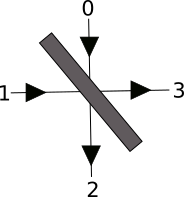
\includegraphics[width=5 cm]{beamsplitter}
\item Easiest to think of a beamsplitter as transforming operators which act on states $\hat{a}^{\dagger}_0\rightarrow \sqrt{1-r}\hat{a}^\dagger_2+i\sqrt{r}\hat{a}^{\dagger}_3$,  $\hat{a}^{\dagger}_1\rightarrow i\sqrt{r}\hat{a}^{\dagger}_2+\sqrt{1-r}\hat{a}^{\dagger}_3$, where $0\le r \le 1$ is the reflectivity
\item Factor of $i$ comes from classical phase shift due to reflection of electromagnetic wave (can be derived from boundary conditions) 
\item Initial and final states are orthogonal for all values of $0\le r \le 1$
\item Most interesting cases occur at $r=\frac{1}{2}$, 50:50 beamsplitter
\begin{align}
\hat{a}^{\dagger}_0\rightarrow \frac{1}{\sqrt{2}}(\hat{a}^{\dagger}_2+i\hat{a}^{\dagger}_3)\\
\hat{a}^{\dagger}_1\rightarrow \frac{1}{\sqrt{2}}(\hat{a}^{\dagger}_3+i\hat{a}^{\dagger}_2)
\end{align}
\item Note: relationships for $\hat{a}$ can be found by taking transpose conjugate of equation
\begin{align}
\hat{a}_0\rightarrow \frac{1}{\sqrt{2}}(\hat{a}_2-i\hat{a}_3)\\
\hat{a}_1\rightarrow \frac{1}{\sqrt{2}}(\hat{a}_3-i\hat{a}_2)
\end{align}
\begin{itemize}
\item Applied to a coherent state in mode $1$ (equation 6.16 in G+K)
\begin{align}
\exp\left[\alpha \hat{a}^\dagger_1-\alpha^* \hat{a}_1\right]\ket{0} \rightarrow \\
\exp\left[\frac{\alpha}{\sqrt{2}}(\hat{a}^{\dagger}_3+i\hat{a}^{\dagger}_2)-\frac{\alpha^*}{\sqrt{2}}(\hat{a}_3-i\hat{a}_2)\right]\ket{0}=\\
\exp\left[\left(\frac{i \alpha}{\sqrt{2}}\right)\hat{a}^{\dagger}_2-\left(\frac{-i \alpha^*}{\sqrt{2}}\right)\hat{a}_2\right]\exp\left[\left(\frac{\alpha}{\sqrt{2}}\right)\hat{a}^{\dagger}_3-\left(\frac{\alpha^*}{\sqrt{2}}\right)\hat{a}_3\right]\ket{0}=\\
\left|\frac{i\alpha}{\sqrt{2}}\right>_2\left|\frac{\alpha}{\sqrt{2}}\right>_3
\end{align}
\item Note that this relies on the fact that operators corresponding to different modes commute
\item Agrees with classical electromagnetic wave expectations $\rightarrow$ there is nothing that coherent states+ beamsplitters can give us which cannot be predicted from classical electromagnatism
\end{itemize}
\item What about a squeezed state?
\begin{itemize}
\item Consider squeezed vacuum (using operator from 7.10 of G+K): 
\begin{align}
\exp\left[\frac{1}{2}(\xi^*\hat{a}_1^2-\xi \hat{a}_1^{\dagger 2})\right]\ket{0} \rightarrow \\
\exp\left[\frac{1}{4}(\xi^*(\hat{a}^{\dagger}_3+i\hat{a}^{\dagger}_2)^2-\xi (\hat{a}_3-i\hat{a}_2)^2)\right]\ket{0}=\\
\exp\left[\frac{1}{4}(\xi^*(\hat{a}^{\dagger 2}_3-\hat{a}^{\dagger 2}_2+2i\hat{a}^{\dagger}_3\hat{a}^{\dagger}_2)-\xi (\hat{a}^2_3-\hat{a}^2_2-2i\hat{a}_3\hat{a}_2))\right]\ket{0}
\end{align}
\item Cross terms involving both $2$ and $3$ don't commute with other terms, not possible to factorize into a product state like a coherent state
\item Beamsplitting squeezed light (even squeezed vacuum) results in entanglement
\item If many beamsplitters are chained together, output from squeezed light is hard to calculate classically, Gaussian Boson Sampling
\end{itemize}
\item A more intuitive example: beamsplitting a number state
\begin{itemize}
\item Start with a number state (2.40 of G+K) 
\begin{align}
 \frac{(\hat{a}_0^\dagger)^n}{\sqrt{n!}}\ket{0} \rightarrow \\
  \frac{(\hat{a}_2^\dagger+i\hat{a}_3^\dagger)^n}{\sqrt{2^n n!}}\ket{0}=\frac{1}{\sqrt{2^n n!}}\sum_{k=0}^n (i^{n-k})\binom{n}{k}(\hat{a}_2^\dagger)^k(\hat{a}_3^\dagger)^{n-k}\ket{0}=\\
  \frac{1}{\sqrt{2^n n!}}\sum_{k=0}^n (i^{n-k})\binom{n}{k} \sqrt{k!(n-k)!}\ket{k}_2\ket{n-k}_3=  \\
 \frac{1}{\sqrt{2^n }}\sum_{k=0}^n (i^{n-k})\frac{n!}{k!(n-k)!} \sqrt{\frac{k!(n-k)!}{n!}}\ket{k}_2\ket{n-k}_3=\\
\sum_{k=0}^n (i^{n-k})\sqrt{  \frac{1}{2^n }\binom{n}{k}} \ket{k}_2\ket{n-k}_3
\end{align}
\item Normalized superpostion of all ways photons can be reflected, normalized state still has $n$ total photons always
\item Very entangled, state of one channel completely determined by state of the other
\end{itemize}
\item What if we put a photon in each input: Hong-Ou-Mandel
\begin{itemize}
\item One photon in each input
\begin{align}
\hat{a}^\dagger_0\hat{a}^\dagger_1\ket{0}\rightarrow\\
\frac{1}{2}(\hat{a}^{\dagger}_2+i\hat{a}^{\dagger}_3)(\hat{a}^{\dagger}_3+i\hat{a}^{\dagger}_2)\ket{0}=
\frac{1}{2}(i\hat{a}^{\dagger 2}_2+i\hat{a}^{\dagger 2}_3+\hat{a}^{\dagger}_2\hat{a}^{\dagger}_3-\hat{a}^{\dagger}_3\hat{a}^{\dagger}_2)\ket{0}=\\
\frac{1}{2}(i\hat{a}^{\dagger 2}_2+i\hat{a}^{\dagger 2}_3)\ket{0}
\end{align}
\item Last line relies on fact that creation in different modes commutes
\item Never see one photon in each direction, interference effect from Bosonic statistics, very different from classical balls bouncing off a peg
\item Note that this only works if phtons are \textbf{perfectly} indistinguishable, any difference (arrival time, frequency, polarisation, etc...) and the cancellation will not occur completely
\item Good way to test if photons are distinguishable $\rightarrow$ classical statistics, indistinguishable $\rightarrow$ Hong-Ou-Mandel, partially distinguishable gives something in between
\item If we chain a lot of these together (and photons are indistinguishable) we get Boson sampling, output hard to calculate classically
\end{itemize}
\end{itemize}

\section{Interferometers}
\begin{itemize}
\item Successive beamsplitters one after another  (with mirrors to redirect beams)

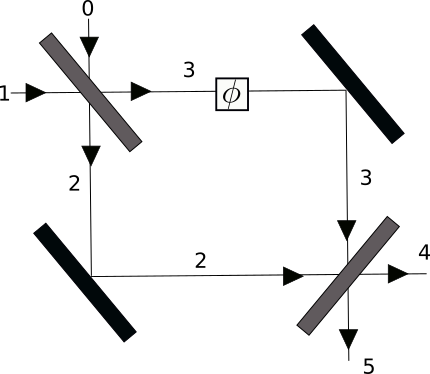
\includegraphics[width=5 cm]{Interferometer}
\item Coherent states in this setting give results for classical EM waves (interference isn't fundamentally quantum water waves interfere for instance)
\item But what about a single photon in a beamsplitter?
\begin{itemize}
\item Interference is between possible paths, not physical objects, still see interference
\begin{align}
\hat{a}^\dagger_0\ket{0}\rightarrow \frac{1}{\sqrt{2}}(\hat{a}^{\dagger}_2+i\hat{a}^{\dagger}_3)\ket{0}\rightarrow\\
\frac{1}{2}(\hat{a}^{\dagger}_4+i\hat{a}^{\dagger}_5-\hat{a}^{\dagger}_4+i\hat{a}^{\dagger}_5)\ket{0}=\hat{a}^\dagger_5\ket{0}
\end{align}
\item Applying beamsplitter twice to a single mode returns a single mode
\item Like with waves, we can apply a phase shift to photon on one arm (by changing length for example) to change outcome:
\begin{align}
\hat{a}^\dagger_0\ket{0}\rightarrow \frac{1}{\sqrt{2}}(\hat{a}^{\dagger}_2+i\hat{a}^{\dagger}_3)\ket{0}\rightarrow\\ 
\frac{1}{\sqrt{2}}(\hat{a}^{\dagger}_2+i\exp(i \phi)\hat{a}^{\dagger}_3)\ket{0} \rightarrow \\
\frac{1}{2}(\hat{a}^{\dagger}_4+i\hat{a}^{\dagger}_5-\exp(i \phi)\hat{a}^{\dagger}_4+i\exp(i \phi)\hat{a}^{\dagger}_5)\ket{0}=\\
\frac{1}{2}\left[(1+\exp(i \phi))\hat{a}^\dagger_5- (1-\exp(i \phi))\hat{a}^\dagger_4\right]\ket{0}
\end{align}
\end{itemize}
\item What if we block one path (path 3)?

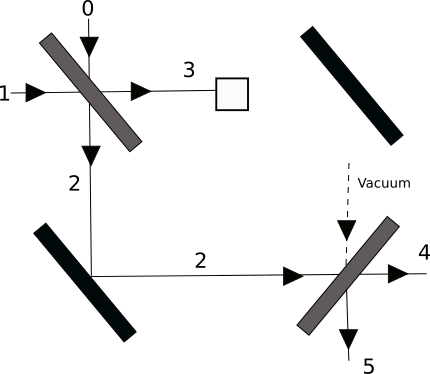
\includegraphics[width=5 cm]{blocked_path}
\begin{itemize}
\item Intermediate state $ \frac{1}{\sqrt{2}}(\hat{a}^{\dagger}_2+i\hat{a}^{\dagger}_3)\ket{0}$ two options each with $50\%$ probability
\begin{enumerate}
\item Photon is in path $3$, is absorbed, end in $\ket{0}$ state, no photon detected anywhere
\item Photon is in path $2$, passes through, state becomes $\hat{a}^{\dagger}_2\ket{0}$, applying second beam splitter leads to $50\%$ chance to be in $4$ or $5$
\end{enumerate}
\item If I detect a photon in path $5$ ($25\%$ overall probability) I know there must be an object in the way \textbf{without} the photon interacting with the object
\item ``Interaction-free'' measurement
\end{itemize}
\item This allows for something which cannot be done classically imagine the following (somewhat artificial) scenario:
\begin{itemize}
\item I have some number of bombs which are triggered by photons, but some of them are faulty
\item The faulty ones simply let the photon pass through (this is the bit which is fairly artificial)
\item The non-faulty ones will explode if a photon tries to pass through
\item I have a bomb-proof apparatus (so ok if I explode some); I want some which are unexploded, but I know are good
\end{itemize}
\item Classically this is impossible, testing will explode the bomb, but quantum mechanically....
\begin{itemize}
\item I can place the bomb on path $3$, 
\item If faulty: the photon arrives on path $5$ with $100\%$ probability (assuming everything is perfect)
\item If functional: 
\begin{enumerate}
\item Explodes with $50\%$ probability (photon took path $3$), 
\item Arrives on path $5$ with $25\%$ probability (took path $2$ and did not reflect on second beamsplitter; indistinguishable from faulty but we can try again)
\item Arrives on path $4$ with $25\%$ probability (took path $2$ but did reflect on second beamsplitter, only possible if bomb works, but no photon has ever interacted with it)
\end{enumerate}
\item A single shot with each bomb will identify a quarter of the functional ones without detonating them (but blow up half)
\end{itemize}
\end{itemize}





\end{document}